% =============================================================================
% COPYRIGHT AND DISCLAIMER
% =============================================================================
% This file is provided as a convenience template for competition participants.
% By using it, you accept full responsibility for compliance with all applicable
% copyright, licensing, and usage rules of the Association for Computing
% Machinery (ACM) and of any LaTeX packages you load (including, without
% limitation, the "acmart" document class and related ACM materials).
%
% Consult ACM's official publication, template, and copyright policies before
% using this setup for any purpose other than this competition. Do not assume
% that this template may be reused, redistributed, or submitted elsewhere
% without independently verifying ACM's current rules.
%
% Use of the "acmart" class, the "sigconf" option, or ACM-style formatting in
% this template does NOT mean that this report, this competition, its organizers,
% or any resulting PDF is sponsored, endorsed, affiliated with, or published by
% ACM. ACM trademarks and branding remain the property of ACM.
%
% Template packages live in preamble.tex.
% Citations live in main.bib. Edit this file with your paper content.
% =============================================================================

\documentclass[sigconf]{acmart}
% =============================================================================
% Template setup — participants normally do not edit this file.
% Author content belongs in main.tex; citations belong in main.bib.
% \documentclass lives in main.tex so Overleaf does not treat this file as root.
% =============================================================================

% --- Competition / non-ACM-submission friendly rights metadata -------------
\setcopyright{none}
\settopmatter{printacmref=false}
\acmConference[Kaggle Competition]{Filament Segmentation Challenge}{2026}{\href{https://www.kaggle.com/competitions/filament-segmentation-2026}{kaggle.com/competitions/filament-segmentation-2026}}
\acmBooktitle{Competition Report}
\acmDOI{}
\acmISBN{}

% --- Author guidance text --------------------------------------------------
% \guide{...} is gray italic while \guideStyletrue; omitted from the PDF if false.
% Flip the switch in main.tex after % =============================================================================
% Template setup — participants normally do not edit this file.
% Author content belongs in main.tex; citations belong in main.bib.
% \documentclass lives in main.tex so Overleaf does not treat this file as root.
% =============================================================================

% --- Competition / non-ACM-submission friendly rights metadata -------------
\setcopyright{none}
\settopmatter{printacmref=false}
\acmConference[Kaggle Competition]{Filament Segmentation Challenge}{2026}{\href{https://www.kaggle.com/competitions/filament-segmentation-2026}{kaggle.com/competitions/filament-segmentation-2026}}
\acmBooktitle{Competition Report}
\acmDOI{}
\acmISBN{}

% --- Author guidance text --------------------------------------------------
% \guide{...} is gray italic while \guideStyletrue; omitted from the PDF if false.
% Flip the switch in main.tex after % =============================================================================
% Template setup — participants normally do not edit this file.
% Author content belongs in main.tex; citations belong in main.bib.
% \documentclass lives in main.tex so Overleaf does not treat this file as root.
% =============================================================================

% --- Competition / non-ACM-submission friendly rights metadata -------------
\setcopyright{none}
\settopmatter{printacmref=false}
\acmConference[Kaggle Competition]{Filament Segmentation Challenge}{2026}{\href{https://www.kaggle.com/competitions/filament-segmentation-2026}{kaggle.com/competitions/filament-segmentation-2026}}
\acmBooktitle{Competition Report}
\acmDOI{}
\acmISBN{}

% --- Author guidance text --------------------------------------------------
% \guide{...} is gray italic while \guideStyletrue; omitted from the PDF if false.
% Flip the switch in main.tex after \input{preamble}.
%
% Do not use \guide{...} for \email{...}.
\usepackage{xcolor}
\newif\ifguideStyle
\guideStyletrue
\newcommand{\guide}[1]{%
\ifguideStyle
{\color{gray!65}\itshape #1}%
\fi
}

% --- Math ------------------------------------------------------------------
% Do NOT load amssymb (or amsfonts): acmart already loads newtxmath, which
% defines the same symbols (e.g. \Bbbk) and causes a conflict on Overleaf.
% amsmath is already provided by acmart; mathtools extends it.
\usepackage{mathtools}

% --- Figures ---------------------------------------------------------------
% graphicx is already loaded by acmart
\usepackage{subcaption}

% --- Tables ----------------------------------------------------------------
% booktabs is already loaded by acmart
\usepackage{tabularx}
\usepackage{multirow}

% --- Bibliography style is set in main.tex (ACM-Reference-Format) ----------
.
%
% Do not use \guide{...} for \email{...}.
\usepackage{xcolor}
\newif\ifguideStyle
\guideStyletrue
\newcommand{\guide}[1]{%
\ifguideStyle
{\color{gray!65}\itshape #1}%
\fi
}

% --- Math ------------------------------------------------------------------
% Do NOT load amssymb (or amsfonts): acmart already loads newtxmath, which
% defines the same symbols (e.g. \Bbbk) and causes a conflict on Overleaf.
% amsmath is already provided by acmart; mathtools extends it.
\usepackage{mathtools}

% --- Figures ---------------------------------------------------------------
% graphicx is already loaded by acmart
\usepackage{subcaption}

% --- Tables ----------------------------------------------------------------
% booktabs is already loaded by acmart
\usepackage{tabularx}
\usepackage{multirow}

% --- Bibliography style is set in main.tex (ACM-Reference-Format) ----------
.
%
% Do not use \guide{...} for \email{...}.
\usepackage{xcolor}
\newif\ifguideStyle
\guideStyletrue
\newcommand{\guide}[1]{%
\ifguideStyle
{\color{gray!65}\itshape #1}%
\fi
}

% --- Math ------------------------------------------------------------------
% Do NOT load amssymb (or amsfonts): acmart already loads newtxmath, which
% defines the same symbols (e.g. \Bbbk) and causes a conflict on Overleaf.
% amsmath is already provided by acmart; mathtools extends it.
\usepackage{mathtools}

% --- Figures ---------------------------------------------------------------
% graphicx is already loaded by acmart
\usepackage{subcaption}

% --- Tables ----------------------------------------------------------------
% booktabs is already loaded by acmart
\usepackage{tabularx}
\usepackage{multirow}

% --- Bibliography style is set in main.tex (ACM-Reference-Format) ----------


% Guide styling: \guideStyletrue = show gray italic hints; \guideStylefalse = omit them
\guideStylefalse

% --- our additions (packages only; template text below is unchanged) ---
\usepackage{tikz}
\usetikzlibrary{arrows.meta,positioning}
\newcommand{\todo}[1]{\textcolor{red}{[TODO: #1]}}
\newcommand{\dpq}{$\Delta$PQ}
\setlength{\emergencystretch}{1em} % absorb three overfull lines from unbreakable tokens

\begin{document}

\title{A P2/stride-2 YOLO detector, crop refiner and agreement-calibrated keep rule for filament instance segmentation}
\subtitle{A Solution to the Solar Filament Segmentation Challenge 2026} % DO NOT CHANGE

\author{Abhimanyu R B}
\affiliation{%
\institution{Anukriti AI}
\city{Trivandrum}
\country{India}
}
\email{abhi@anukritiai.com}

\begin{abstract}
This report describes our solution to the Solar Filament Segmentation Challenge~2026, a Kaggle competition on automatic segmentation of solar filaments in GONG H-$\alpha$ observations.
We segment filaments on $2048^2$ images with a YOLO11s-seg detector extended by a P2 level with stride-2 mask prototypes, 4-flip consensus, a ResNet18 U-Net crop refiner trained on the detector's own out-of-fold proposals with annotator-averaged soft targets, and a LightGBM keep rule that drops masks a random annotator is unlikely to have drawn. On leak-free 5-fold out-of-fold (OOF) validation over all 707 training files the final pipeline reaches a pooled per-record Panoptic Quality (PQ) of \textbf{0.4590} (public leaderboard 0.39). Human annotators agree with each other at only PQ $\approx$0.34; most of the remaining error is annotator disagreement rather than mask quality. Inference runs end-to-end at 2.5\,s per image on one T4 GPU, and the public repository regenerates both selected submissions byte-for-byte.
\end{abstract}

\maketitle

\ifguideStyle
\noindent{\color{gray!65}\itshape
Guide mode is on.}
\par\medskip
\fi

\guide{Please limit your report to four (4) pages, excluding the Acknowledgment and References sections. Throughout this document, please follow these considerations:
\begin{itemize}
\item Do not alter any text that is currently in black color (except for the emails under authors' name).
\item Replace all gray text with your own.
\item When you are done with the report, please replace \texttt{\textbackslash guideStyletrue} with \texttt{\textbackslash guideStylefalse}, to remove any gray text. Alternatively, you can remove any text wrapped in \texttt{\textbackslash guide\{\}},
\item Be as succinct as possible, and only provide details regarding your own work. For example, there is no need to discuss what solar filaments are, or why filament segmentation matters.
\item If you must, you can add extra sections.
\end{itemize}}

% ==================================== %
% INTRODUCTION %
% ==================================== %
\section{Introduction}
This report goes over the details of our submitted solution to the Solar Filament Segmentation Challenge~2026 \cite{filament-segmentation-2026}. The challenge, launched on July~10,~2026, is organized by the Earth-Space AI Research (ESAIR) Lab\footnote{\href{https://www.esairlab.com/home}{www.esairlab.com/}}. This challenge utilizes the MAGFiLO dataset for evaluation of the segmentation algorithms \cite{ahmadzadeh2024dataset}.
Our approach is a detector-first instance pipeline (Section~\ref{sec:methodology}) chosen for its recall on thin, low-contrast structures, followed by a crop refiner for mask extent and a learned selection step tuned to the per-annotator-record scoring of the challenge. Every design decision was tested under a pre-registered, leak-free 5-fold protocol with paired bootstrap uncertainty (Section~\ref{sec:evaluation}); the code, SHA-pinned weights and a notebook that regenerates the selected submission are in the public repository.\footnote{\url{https://github.com/Abm32/solar-filament-2026}}

% ==================================== %
% METHODOLOGY %
% ==================================== %
\section{Methodology}\label{sec:methodology}

\subsection{Task, metric and data splits}
\textbf{Data.} 707 training files with 1154 annotator records and 8199 polygons (411 files have one record, 145 two, 151 three); 180 test images. No pre-processing is applied to the images beyond resizing to 1024\,px for the detector; the refiner and the output masks work at native 2048\,px.
\textbf{Metric.} Panoptic Quality \cite{kirillov2019panoptic} with IoU$>$0.5 matching, where each prediction set is matched separately against every annotator record and TP/FP/FN are pooled over all (image, record) pairs. A filament drawn by $k$ of $n$ annotators and predicted with IoU $s$ thus earns $k$ TP and $n-k$ FP, so predicting it pays only if roughly $k/n > \mathrm{PQ}/(2s)\approx0.31$: the target is ``would a random annotator draw this'', not ``is this a filament''. Our scorer reproduces the host self-evaluation notebook exactly (identical TP/FP/FN on all 707 files).
\textbf{Splits.} We use a 5-fold out-of-fold (OOF) split by file (141--142 files per fold; files from the same observing day are kept in one fold). Every file is predicted by detector, refiner and keep-rule models that never saw it; the refiner and the keep rule are refit per fold, so refined OOF numbers are leak-free. The final models are refit on all 707 files with the same recipes. No validation subset is held out from the test images; the public leaderboard was not used for model selection (Section~\ref{sec:lb}).

\subsection{Pipeline}
Figure~\ref{fig:pipeline} shows the six inference stages; Figure~\ref{fig:examples} shows OOF outputs.

\begin{figure}[t]\centering
\begin{tikzpicture}[font=\scriptsize, node distance=2.3mm,
  box/.style={draw, rounded corners=1pt, align=center, inner sep=2pt, minimum height=5.5mm, text width=23mm},
  arr/.style={-{Latex[length=1.4mm]}, thick}]
\node[box] (img) {H$\alpha$ image\\$2048^2$ $\to$ 1024\,px};
\node[box, right=of img] (det) {(1) p2first\\YOLO11s-seg, 4 flips};
\node[box, right=of det] (con) {(2) flip consensus\\IoU 0.5 clusters};
\node[box, below=of con] (own) {(3) pixel ownership\\(score order)};
\node[box, left=of own] (ref) {(4) crop refiner\\ResNet18 U-Net, 256\,px};
\node[box, left=of ref] (keep) {(5) MIN200 +\\LightGBM demote};
\node[box, below=of keep] (out) {(6) RLE export\\+ validator};
\draw[arr] (img) -- (det); \draw[arr] (det) -- (con); \draw[arr] (con) -- (own);
\draw[arr] (own) -- (ref); \draw[arr] (ref) -- (keep); \draw[arr] (keep) -- (out);
\end{tikzpicture}
\caption{Inference pipeline. Stages (1)--(3) produce pixel-disjoint proposals with consensus scores; (4) re-predicts each mask at full resolution; (5) decides which masks to keep; (6) writes COCO RLE.}
\label{fig:pipeline}
\end{figure}

\textbf{(1) Detector: ``p2first'' YOLO11s-seg.} We add a P2 level to YOLO11s-seg \cite{ultralytics2024yolo11} (Upsample $\to$ Concat with backbone P2 $\to$ C3k2[128]) and place it \emph{first} in the Segment head inputs [P2,P3,P4,P5]. Because Ultralytics builds mask prototypes from the first input, this gives stride-2 prototypes (512$\times$512 at 1024 input) plus stride-4 detection, which matters for thin, small filaments. Init: COCO YOLO11s-seg with head tensors re-indexed (509/639 tensors transfer). Training: single class, imgsz 1024, batch 4, 80 epochs at mask\_ratio 2 then 20 epochs at mask\_ratio 1 (AdamW $10^{-4}$), seed 42; one annotator record = one training image. Input: the 8-bit JPEG read as grayscale, replicated to three channels and scaled to $[0,1]$; augmentation: mosaic 0.3 (off for the last 5 epochs), brightness (hsv\_v) 0.3, rotation $\pm10^\circ$, translate 0.1, scale 0.3, no flips. At inference: box IoU 0.3, retina masks, agnostic NMS, score floor 0.1.

\textbf{(2) 4-flip TTA and consensus.} Inference on identity, H, V and HV flips; masks are clustered across views (anchor = highest score, IoU 0.5); cluster score = sum of view scores / 4. \textbf{(3) Pixel ownership.} Score-ordered ownership makes instances pixel-disjoint (required by the host).

\textbf{(4) Crop refiner.} A ResNet18 \cite{he2016resnet} U-Net \cite{ronneberger2015unet} on 256-px proposal-centred crops (context 1.8, 4-flip TTA) re-predicts each mask at full 2048 resolution, clamped to a 7$\times$7 dilation of its seed. It is trained on the detector's \emph{own OOF proposals} in two stages: (A) 8 epochs on GT crops (lr $3\cdot10^{-4}$) from an ImageNet encoder, (B) 12 epochs on proposals matched to GT (IoU$\ge$0.3), 0.5 BCE + 0.5 Dice, AdamW $10^{-4}$, cosine schedule, batch 16. Crops are grayscale$/255$ replicated to three channels and ImageNet mean/std normalised; augmentation: random $90^\circ$ rotation, horizontal flip, gamma 0.85--1.2, gain 0.9--1.1. Stage B uses \emph{soft targets}: the target is the per-pixel mean, over the $R$ annotator records, of the GT mask each record matched to the proposal (0 for records without a match), so the refiner learns agreement-weighted extent. Mask threshold $t=0.50$, detection cut $c=0.30$.

\textbf{(5) MIN200 + demote rule.} Masks below 200\,px are dropped. A LightGBM \cite{ke2017lightgbm} regressor on 28 per-candidate features (consensus and member scores, view support, ownership retention, refined-probability statistics, area, elongation, width, disk position, contrast, disk statistics, neighbour and per-file counts) predicts for each kept mask $j$ the expected per-record matched quality $\hat y_j\approx q_j s_j$, where $q_j$ is the fraction of records that match it and $s_j$ the mean matched IoU. Since $\mathrm{PQ}=\sum q s/(\mathrm{TP}+\tfrac12\mathrm{FP}+\tfrac12\mathrm{FN})$, adding mask $j$ raises PQ iff $q_j s_j > \mathrm{PQ}/2$; the optimal keep set is therefore a threshold on $\hat y$ at $\lambda/2$, with $\lambda$ the fixed point $\lambda=\mathrm{PQ}(\{j:\hat y_j>\lambda/2\})$ found by Dinkelbach iteration ($\lambda=0.4587$ on pooled cross-fitted OOF). Only demotion is used (promoting masks below $c$ gave +0.0001). On OOF it removes 9.3\% of masks (4686$\to$4248), on test 8.3\%.

\textbf{(6) Export.} Native 2048 masks, COCO RLE, validated (180 ids, non-overlap, full decode) before writing.

\begin{figure}[t]\centering
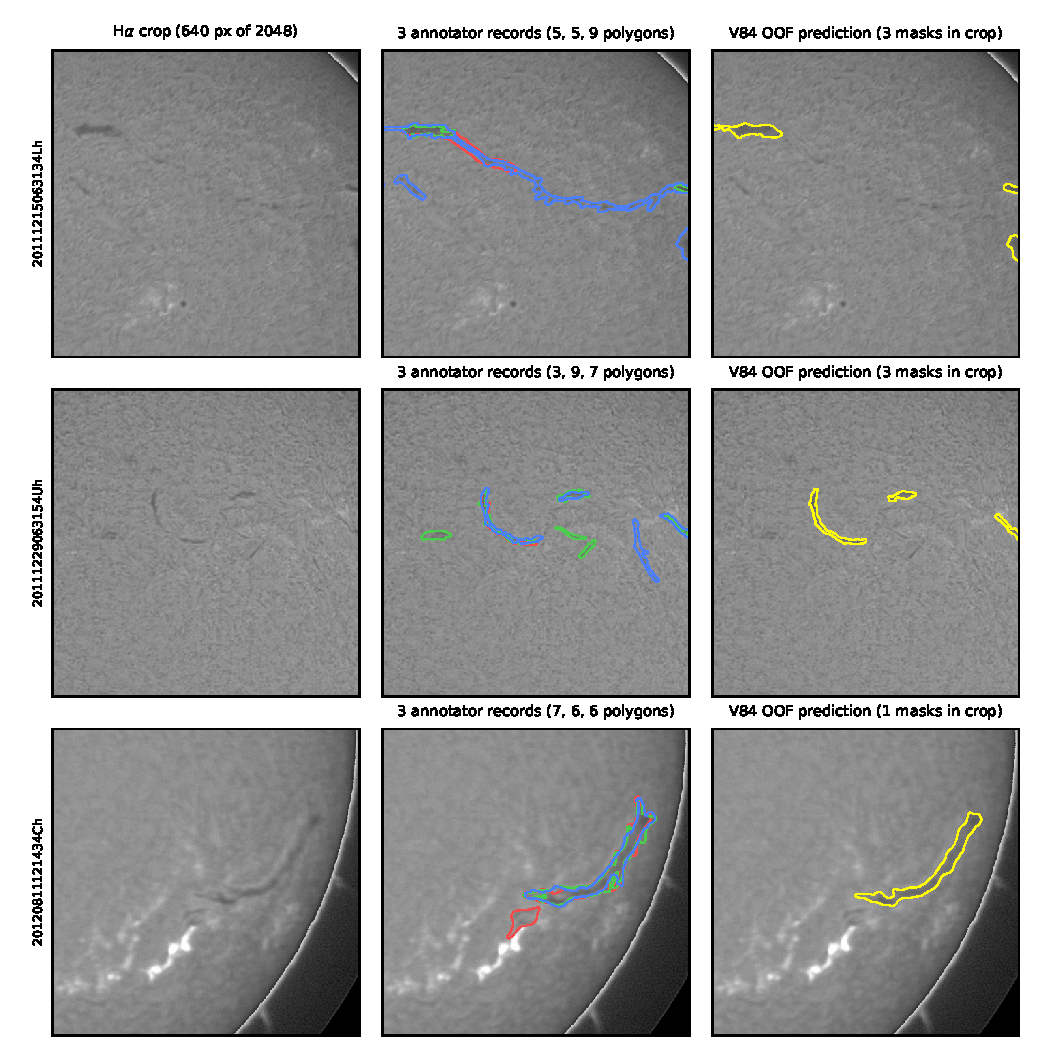
\includegraphics[width=\columnwidth]{figures/examples.pdf}
\caption{OOF examples on three 3-record training files (640-px crops), chosen as the median-density 3-record files, not by score. Left: H$\alpha$ crop. Middle: the three annotator records (one colour each); note how often records disagree on which dark structures are filaments and where they end. Right: the V84 OOF prediction (yellow).}
\label{fig:examples}
\end{figure}

% ==================================== %
% EVALUATION %
% ==================================== %
\section{Evaluation}\label{sec:evaluation}

\subsection{Evaluation strategy}
Each experiment is \emph{pre-registered}: arms, metric and a mechanical CONTINUE/KILL gate are written and hashed (sha256) before any number exists. Comparisons use a paired file-level bootstrap (2000 resamples) over the 707 OOF files and report \dpq, 95\% CI, $P(\Delta>0)$ and per-fold signs. Typical gate: pooled \dpq$\ge$+0.010 (screens) or $\ge$+0.005 (final bundle), $P\ge0.90$, $\ge$4/5 folds positive; KILL if \dpq$<$+0.005. Seed and retraining noise are measured, not assumed (detector seed noise $-0.005$ on fold 0; pooled 5-fold detector retrain +0.0015; refiner retraining noise $\approx$0.0001; refiner seed spread up to 0.004). The public leaderboard shows two decimals on $\sim$90 images and cannot resolve effects of this size, so it was not used for selection.

\subsection{Results}
\begin{table}[t]\centering\small
\caption{5-fold OOF, 707 files, pooled per-record PQ. Baseline = V65 deployed path (p2first + r3 refiner, $t$0.45/$c$0.30) with leak-free 5-fold refiner. Paired bootstrap vs baseline, 95\% CI.}
\label{tab:main}
\setlength{\tabcolsep}{3pt}
\resizebox{\columnwidth}{!}{\begin{tabular}{lcccc}
\toprule
pipeline & PQ & SQ & TP/FP/FN & \dpq\ [95\% CI] \\
\midrule
V65 path (baseline) & 0.4539 & .685 & 5270/2444/2929 & -- \\
\textbf{V84 (final)} & \textbf{0.4590} & .688 & 5050/1881/3149 & \textbf{+0.0050} [+.0024,+.0077] \\
\midrule
only soft targets & 0.4550 & .685 & & +0.0011 [+.0001,+.0021] \\
only $t$0.50 & 0.4546 & .686 & & +0.0007 [$-$.0001,+.0015] \\
only MIN200 & 0.4560 & .685 & & +0.0021 [+.0014,+.0029] \\
only demote & 0.4569 & .687 & & +0.0030 [+.0007,+.0053] \\
V84 $-$ MIN200 & 0.4590 & .688 & & +0.0051 [+.0023,+.0077]\\
V84 $-$ demote & 0.4567 & .686 & & +0.0028 [+.0013,+.0044]\\
\bottomrule
\end{tabular}}
\end{table}

Table~\ref{tab:main} gives the final comparison. The V84 bundle gains \dpq\ = +0.0050, CI [+0.0024, +0.0077], $P(\Delta>0)=0.9995$, positive on 5/5 folds (+.0057, +.0097, +.0028, +.0027, +.0045). It met its pre-registered +0.005 bar by only 0.00004, so we expect $\approx$+0.005$\pm$0.003 on test, not a certain gain. Single components sum to +0.0069; the bundle keeps 73\%. The demote rule is the largest marginal component and makes MIN200 redundant (MIN200 is kept as a harmless export default). Both V65 and V84 are our two selected submissions; both score \textbf{0.39} on the public leaderboard.

Earlier milestones (direct detector, 707 files): baseline YOLO11s-seg 0.3856 $\to$ p2first 0.4060 (\dpq\ +0.0204 [+0.0151, +0.0256], 5/5 folds; small-object recall 0.411$\to$0.460). The crop refiner adds $\approx$+0.04--0.06 PQ on top of any detector, mostly via SQ (0.657$\to$0.689).

\textbf{Negative results: the refiner absorbs detector gains.} Table~\ref{tab:neg} lists pre-registered experiments killed by their gates. A recurring finding is that improvements that are clear on the direct detector vanish after refinement: the refiner already fixes mask geometry, so detector gains must come from \emph{instance selection}, not extent. From V76 on, every detector change had to pass a refined-pipeline gate.

\begin{table}[t]\centering\small
\caption{Selected pre-registered negatives. Direct = detector only; refined = through the refiner and keep rule. 141 held-out files (fold-0 screens), except refiner variants, re-scorer, pooled selector, ownership, SSL and spine-net instances (707-file 5-fold).}
\label{tab:neg}
\setlength{\tabcolsep}{2.5pt}
\resizebox{\columnwidth}{!}{\begin{tabular}{lll}
\toprule
change & direct \dpq & refined \dpq\ [95\% CI] \\
\midrule
imgsz 1280 & +0.0143 & $-$0.0029 [$-$.013,+.007] \\
thin labels ($-$1 px polygons) & +0.0272 & $-$0.0017 [$-$.010,+.007] \\
noisy student (unlab.\ GONG) & +0.0106 & +0.0007 [$-$.010,+.011] \\
label transfer $\pm$1/2/5 min & $-$.011/+.001/$-$.006 & not run (killed) \\
2-detector ensemble & +0.0063 & +0.0016 [$-$.006,+.009] \\
pooled 3-detector selector & -- & +0.0003 [$-$.003,+.004] \\
ownership by refiner prob.\ (argmax) & -- & $-$0.0017 (fails all bars) \\
refiner: union targets & -- & $-$0.0195 [$-$.026,$-$.013] \\
refiner: quality-weighted & -- & $-$0.0000 [$-$.002,+.002] \\
refiner: crop512 / RN34 / dil15 & -- & +.0000 / +.0006 / +.0006 \\
refiner: in-domain SSL init (MIM / MoCo) & -- & $-$0.0011 / $-$0.0027 \\
learned re-scorer (agreement) & +0.0161 & $-$0.0099 [$-$.018,$-$.002] \\
spine-first dense U-Net (no detector) & -- & 0.4333 standalone; fusion +0.0002 \\
spine-net instances via refiner + keep rule & -- & +0.0011 [$-$.001,+.003] \\
limb-darkening-divided detector input & $-$0.0022 & $-$0.0073 [$-$.018,+.003] \\
fine-tune on hard-annotator records & -- & $-$0.0138 [$-$.028,+.001] (hard subset) \\
annotator-group-conditioned refiner & -- & $-$0.0030 [$-$.012,+.006] (group 01); oracle style $-$0.0002 \\
\bottomrule
\end{tabular}}
\end{table}
Other closed lines: Mask R-CNN, Mask2Former, DenseCRF, BCE+Focal+\allowbreak Dice loss, YOLO11m, size-gated refiner ($-$0.014), 1-px erosion of refined masks ($-$0.024). Soft targets (+0.0019, fold 0) and the keep rule (+0.0030, 707 files) failed their \emph{individual} gates and were only adopted as a re-registered bundle.

\subsection{Host evaluation plots}
\begin{figure*}[t]\centering
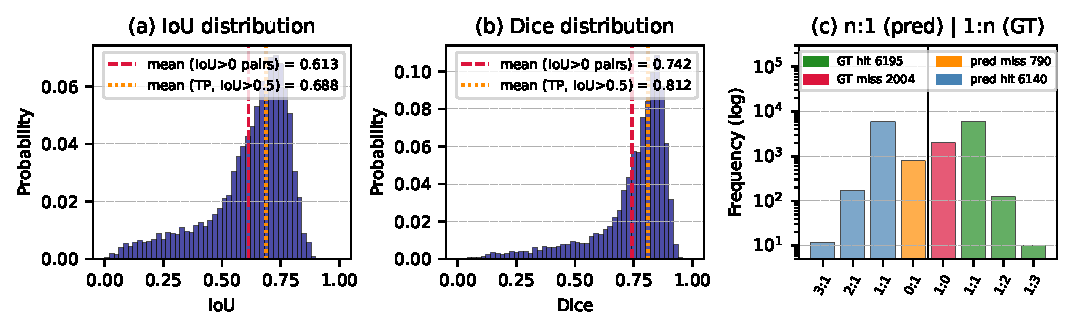
\includegraphics[width=0.86\textwidth]{figures/host_plots.pdf}
\caption{Host self-evaluation plots for the V84 pipeline on 5-fold OOF predictions (707 training files, 8199 GT polygons over all records; PQ 0.4590 reproduced). Logic mirrors the host notebook (\texttt{plot\_distribution}, \texttt{plot\_m2n\_counts}): all GT--prediction pairs with IoU$>$0 per annotator record. (a) IoU, (b) Dice (=2IoU/(1+IoU) per pair), (c) number of overlapping partners per GT (1:$n$, right) and per prediction ($n$:1, left).}
\label{fig:host}
\end{figure*}
Figure~\ref{fig:host} shows the three required distributions on OOF predictions. Over all overlapping pairs the mean IoU is 0.613 (Dice 0.742); over matched pairs (IoU$>$0.5) 0.688 (Dice 0.812). The IoU mass sits at 0.65--0.80 and drops sharply above 0.85: annotators' own boundaries disagree at that level (human SQ $\approx$0.63). Topology errors are rare: 134 of 8199 GT (1.6\%) overlap $\ge$2 predictions (fragmentation) and 187 prediction-record pairs (2.7\%) overlap $\ge$2 GT (over-merging); 1:1 dominates on both sides. The 2004 GT with no overlapping prediction are mostly filaments drawn by a single annotator (below).

\subsection{Error analysis and the annotator-disagreement ceiling}
A stage-wise decomposition of the 3149 OOF FN shows that 65\% had a candidate with IoU$>$0.5 somewhere in the pipeline that was dropped (28\% by the score cut, 19\% by pixel ownership to a higher-scored neighbour, 7\% by the demote rule), 21\% were shape near-misses (IoU 0.3--0.5) and only 14\% had no usable candidate; 95\% of the latter were drawn by a single annotator. Of the 1881 FP, 41\% are another annotator's TP on the same image and cannot be removed without losing that TP. The hardest ground truth is low-contrast (lowest quintile: recall 0.33), small ($\le$500\,px: 0.42) and blobby (elongation $<$10: 0.52); recall does not depend on image statistics (site, year, sharpness, disk std all $|\rho|<0.06$).

On the 296 multi-record training files we scored annotators against each other and computed label oracles (all with access to GT, so they are ceilings, not achievable predictors):
\begin{itemize}
\item \textbf{Human vs.\ held-out human:} PQ \textbf{0.340} (SQ 0.634; 1196 ordered pairs). Our direct detector scores 0.411 on the same records, so the model already beats a held-out annotator.
\item \textbf{Oracle predictors} (submit GT masks, scored against all records of the file): union of annotators \textbf{0.663}; one annotator's own masks \textbf{0.605} (best/worst 0.631/0.571); majority/$k\ge2$ \textbf{0.592}. Even perfect masks cap PQ near 0.6--0.67 because records disagree on \emph{which} filaments exist.
\item \textbf{Keep-oracle:} choosing which of our own existing refined masks to keep using the true $q\cdot s$ gives 0.5283 (\textbf{+0.074}); our learned rule realises +0.003 of it. Agreement is weakly predictable from image or refiner evidence (Spearman with true $qs$: 0.59 vs 0.57 for the score alone).
\item Recall on filaments drawn by $\ge$2 annotators is 0.834 vs 0.367 for single-annotator ones; fixing every missed agreed filament would add only +0.030.
\end{itemize}

\subsection{Public leaderboard}\label{sec:lb}
Every clean pipeline we could audit, ours included, loses 0.05--0.07 PQ from local validation to the public board. To test whether this offset is a tunable, we submitted five one-knob perturbations of the V84 export and read each against the same perturbation on the 707-file OOF: dilate 1\,px (public $-$0.02 / OOF $-$0.021), erode 1\,px ($-$0.03 / $-$0.037), $c$=0.20 without demote ($-$0.01 / $-$0.013), $c$=0.40 (0.00 / $-$0.008), fold-0 models instead of all-data fits (0.00). Every knob moved the public board by the amount it moved OOF, so the V84 operating point is also the test optimum and the offset is in the content of the test labels (recall side), not in mask width, thresholds or the all-data refits.

\subsection{Compute and efficiency}
Training on 4$\times$ NVIDIA T4 (one model per GPU; DDP is incompatible with the in-process stride-2 patch). Final all-data detector: 2.4\,h (stage 1, 80 ep) + 2.1\,h (stage 2, 20 ep) = 4.5 GPU-h; all-data refiner 24\,min; LightGBM demote model: seconds on CPU. The full 5-fold OOF protocol costs $\approx$5$\times$ this. \textbf{Inference} (public repository, fresh environment from \texttt{requirements.txt}, 180 test images, one T4): \textbf{2.4\,s per image} end-to-end (4-flip detector at 1024\,px, 4-flip crop refiner, keep rule, RLE), 440\,s wall, flat memory; the regenerated CSV is byte-identical to the submitted file.

\subsection{Strengths, weaknesses and possible improvements}
\textbf{Strengths.} Stride-2 prototypes give the detector small-object recall that generic instance models lacked; the refiner raises SQ above the human-vs-human level; the keep rule is derived from the metric itself and transfers to the test board at the same operating point; every claim carries a CI from a leak-free protocol.
\textbf{Weaknesses.} The final gain over V65 (+0.005) is small and passed its gate narrowly; the all-data refiner and demote model are single fits (refiner seed spread up to 0.004). Thin structures (barbs; agreed filaments narrower than 5\,px: recall 0.60) remain the hardest morphology, and the pipeline predicts one consensus mask per filament, so it cannot score well against records that disagree on extent. The OOF-to-public offset is outside the model's control.
\textbf{Improvements.} The largest measured headroom is predicting inter-annotator agreement (+0.074 keep-oracle), which our 28 features reach only weakly; multi-hypothesis refinement (refine every view member, not only the consensus representative) and an ownership rule that does not let a fatter neighbour swallow a thinner true filament each bound +0.01 on OOF.

\section{Data use and rule compliance}
\begin{itemize}
\item \textbf{Training data:} only the provided training images and labels. No external ground truth of any kind (SWEFil was not used after the host ruling, and no SWEFil-trained artefact is in the pipeline or repository); no test labels or pseudo-labels on test images. Pretrained weights: COCO YOLO11s-seg (Ultralytics), ImageNet ResNet18 (torchvision).
\item \textbf{Inference:} single-image; each test H$\alpha$ image alone (no neighbouring frames, no magnetograms).
\item \textbf{Training-only experiments not in the final pipeline}, run under host rulings: (i) label transfer of training polygons to nearby GONG frames $\pm$1--5 min, excluding any frame within $\pm$1\,h of a test timestamp (discussion thread 748045); (ii) noisy-student pseudo-labelling on unlabelled GONG frames from days excluding all train and test dates $\pm$1 day (thread 744047); (iii) in-domain self-supervised refiner initialisation on the same frames. All were killed by their pre-registered gates (Table~\ref{tab:neg}) and none of these data are used by the submitted models.
\end{itemize}

% ==================================== %
% ACKNOWLEDGMENT %
% ==================================== %
\section{Acknowledgment}\label{sec:acknowledgment}
% Do not change
The organization of the Filament Segmentation Challenge 2026 is partially supported by the U.S. National Science Foundation (NSF) under Grant No. 2209912 and 2433781, directorate for Computer and Information Science and Engineering (CSE), and Office of Advanced Cyberinfrastructure (OAC), and Grant No. 2511630, AST Division Of Astronomical Sciences and MPS Directorate for Mathematical and Physical Sciences.

The Filament Segmentation Challenge 2026 is sponsored by the U.S. National Science Foundation (NSF) National Solar Observatory (NSO).

This work utilizes GONG data obtained by the NSO Integrated Synoptic Program, managed by the National Solar Observatory, which is operated by the Association of Universities for Research in Astronomy (AURA), Inc. under a cooperative agreement with the National Science Foundation and with contribution from the National Oceanic and Atmospheric Administration. The GONG network of instruments is hosted by the Big Bear Solar Observatory, High Altitude Observatory, Learmonth Solar Observatory, Udaipur Solar Observatory, Instituto de Astrofísica de Canarias, and Cerro Tololo Interamerican Observatory.

\bibliographystyle{ACM-Reference-Format}
\bibliography{main}

\end{document}
